\documentclass[10pt]{article}

\usepackage{spheric}
%%%TITLE
\title{A Two-Phase SPH Model for Sediment Laden Flows}
\date{}

%%AFFILIATIONS
\author[$\relax$]{Huabin Shi$^\dagger$}
\author[$\relax$]{Xiping Yu}

\affil[$\relax$]{Tsinghua University, Beijing, China}
\affil[$\relax$]{\email{\dagger}{shihuabin@tsinghua.edu.cn}}


%%DOCUMENT
\begin{document}

\maketitle

%\SelectedTopics{}

%%PLEASE PUT YOUR ABSTRACT HERE
\begin{abstract}
A two-phase SPH model based on a general volume fraction formulation for solid-fluid flows is proposed for sediment motion in free surface flows. Different from the existing SPH two-phase models, in the present model the water and the sediment are treated as two miscible fluids, and the two-fluid system is discretized by a single set of SPH particles, which move with the water velocity and carry properties of the two phases. Turbulence in both the water and sediment phases are dealt with and the particle-turbulence interaction are taken into account. The water is assumed to be weakly compressible while the sediment phase is incompressible. A new equation of state is proposed for the hydrodynamic pressure in the sand-water mixture and a matching strategy of Shepard filtering is adopted to damp the oscillation in pressure.

The model is validated and applied to sand dumping from a line source into a water tank and bed erosion under dam break flows. The computed results are in good agreement with the experimental data. Figure \ref{fig:31-1} shows the distributions of sediment concentration carried by SPH particles in the dumping of fine and coarse sand. Figure \ref{fig:31-2} compares the computational and experimental water free surface and bed profiles under dam break flows. It is shown in the applications that the proposed model promises to be an effective tool for sediment transport in free surface flows.

\begin{figure}[!htb]
\begin{minipage}[b]{0.46\linewidth}
\centering
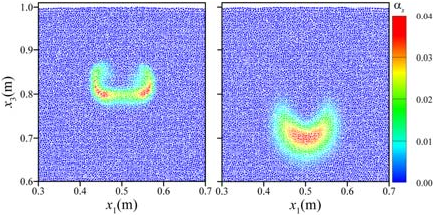
\includegraphics[width=\textwidth]{31-1.pdf}
\caption{Computed sediment concentrations of the SPH particles. Left: Fine sand with a diameter of 0.8 mm; Right: Coarse sand with a diameter of 5.0 mm.}\label{fig:31-1}
\end{minipage}
\begin{minipage}[b]{0.05\linewidth}
~
\end{minipage}
\begin{minipage}[b]{0.46\linewidth}
\centering
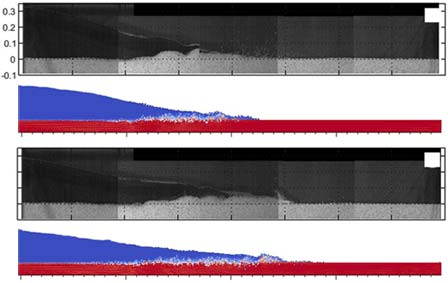
\includegraphics[width=0.8\textwidth]{31-2.png}
\caption{Comparisons between the computed and measured water free surface and bed profiles under dam break flows.}\label{fig:31-2}
\end{minipage}
\end{figure}


\end{abstract}


%%THE END OF ABSTRACT

\addbib

\end{document}
